% Created 2020-03-31 Tue 16:45
% Intended LaTeX compiler: pdflatex
\documentclass[presentation]{beamer}
\usepackage[utf8]{inputenc}
\usepackage[T1]{fontenc}
\usepackage{graphicx}
\usepackage{grffile}
\usepackage{longtable}
\usepackage{wrapfig}
\usepackage{rotating}
\usepackage[normalem]{ulem}
\usepackage{amsmath}
\usepackage{textcomp}
\usepackage{amssymb}
\usepackage{capt-of}
\usepackage{hyperref}
\usetheme{UoB}
\author{Mark Blyth}
\date{}
\title{Numerical continuation in computational biology}
\hypersetup{
 pdfauthor={Mark Blyth},
 pdftitle={Numerical continuation in computational biology},
 pdfkeywords={},
 pdfsubject={},
 pdfcreator={Emacs 26.3 (Org mode 9.1.9)}, 
 pdflang={English}}
\begin{document}

\maketitle

\section{Chapter 1}
\label{sec:org22329bb}
\begin{frame}[label={sec:org7930d66}]{What is computational biology?}
\begin{itemize}
\item Goal: use maths to understand the mechanisms behind living processes
\item Differential equations are used to explain lots of these processes
\begin{itemize}
\item Hodgkin-Huxley: neural dynamics
\item Lotka-Volterra: population dynamics
\item SIR model: epidemic dynamics
\end{itemize}
\end{itemize}
\end{frame}

\begin{frame}[label={sec:org788c7c6}]{Differential equations for biology}
\begin{block}{Ordinary differential equation}
Description of how a system state changes in time
\end{block}

\begin{block}{System state}
Minimal amount of information to describe something's behaviour
\end{block}

\begin{block}{Nonlinear system}
A set of ordinary differential equations, where the change in state doesn't follow a simple proportional relationship
\end{block}
\end{frame}

\begin{frame}[label={sec:org5478950}]{Drawing pictures}
\begin{center}
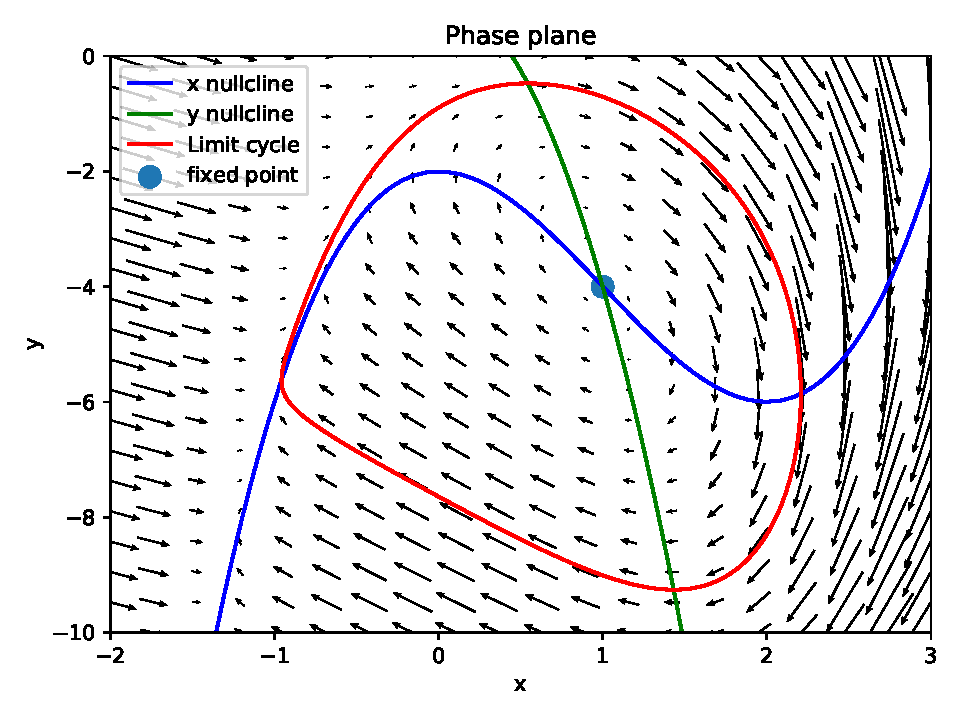
\includegraphics[height=.9\textheight]{./phaseplane.pdf}
\end{center}
\end{frame}

\begin{frame}[label={sec:org6511a4c}]{The role of parameters}
\emph{Every} equation has parameters:
\begin{itemize}
\item Some of these are fixed
\item Some of these we can play with
\end{itemize}

The dynamics of a system necessarily depend on these parameters
\end{frame}

\begin{frame}[label={sec:orga611aa3}]{Bifurcations}
\begin{block}{Bifurcation}
If the dynamics of a system change at some parameter value, a bifurcation is said to have occurred
\end{block}
\vfill

This usually means equilibria or periodic orbits appearing and disappearing -- but not always!
\end{frame}

\begin{frame}[label={sec:org9b099c0}]{Biological bifurcations}
\begin{columns}
\begin{column}{0.5\columnwidth}
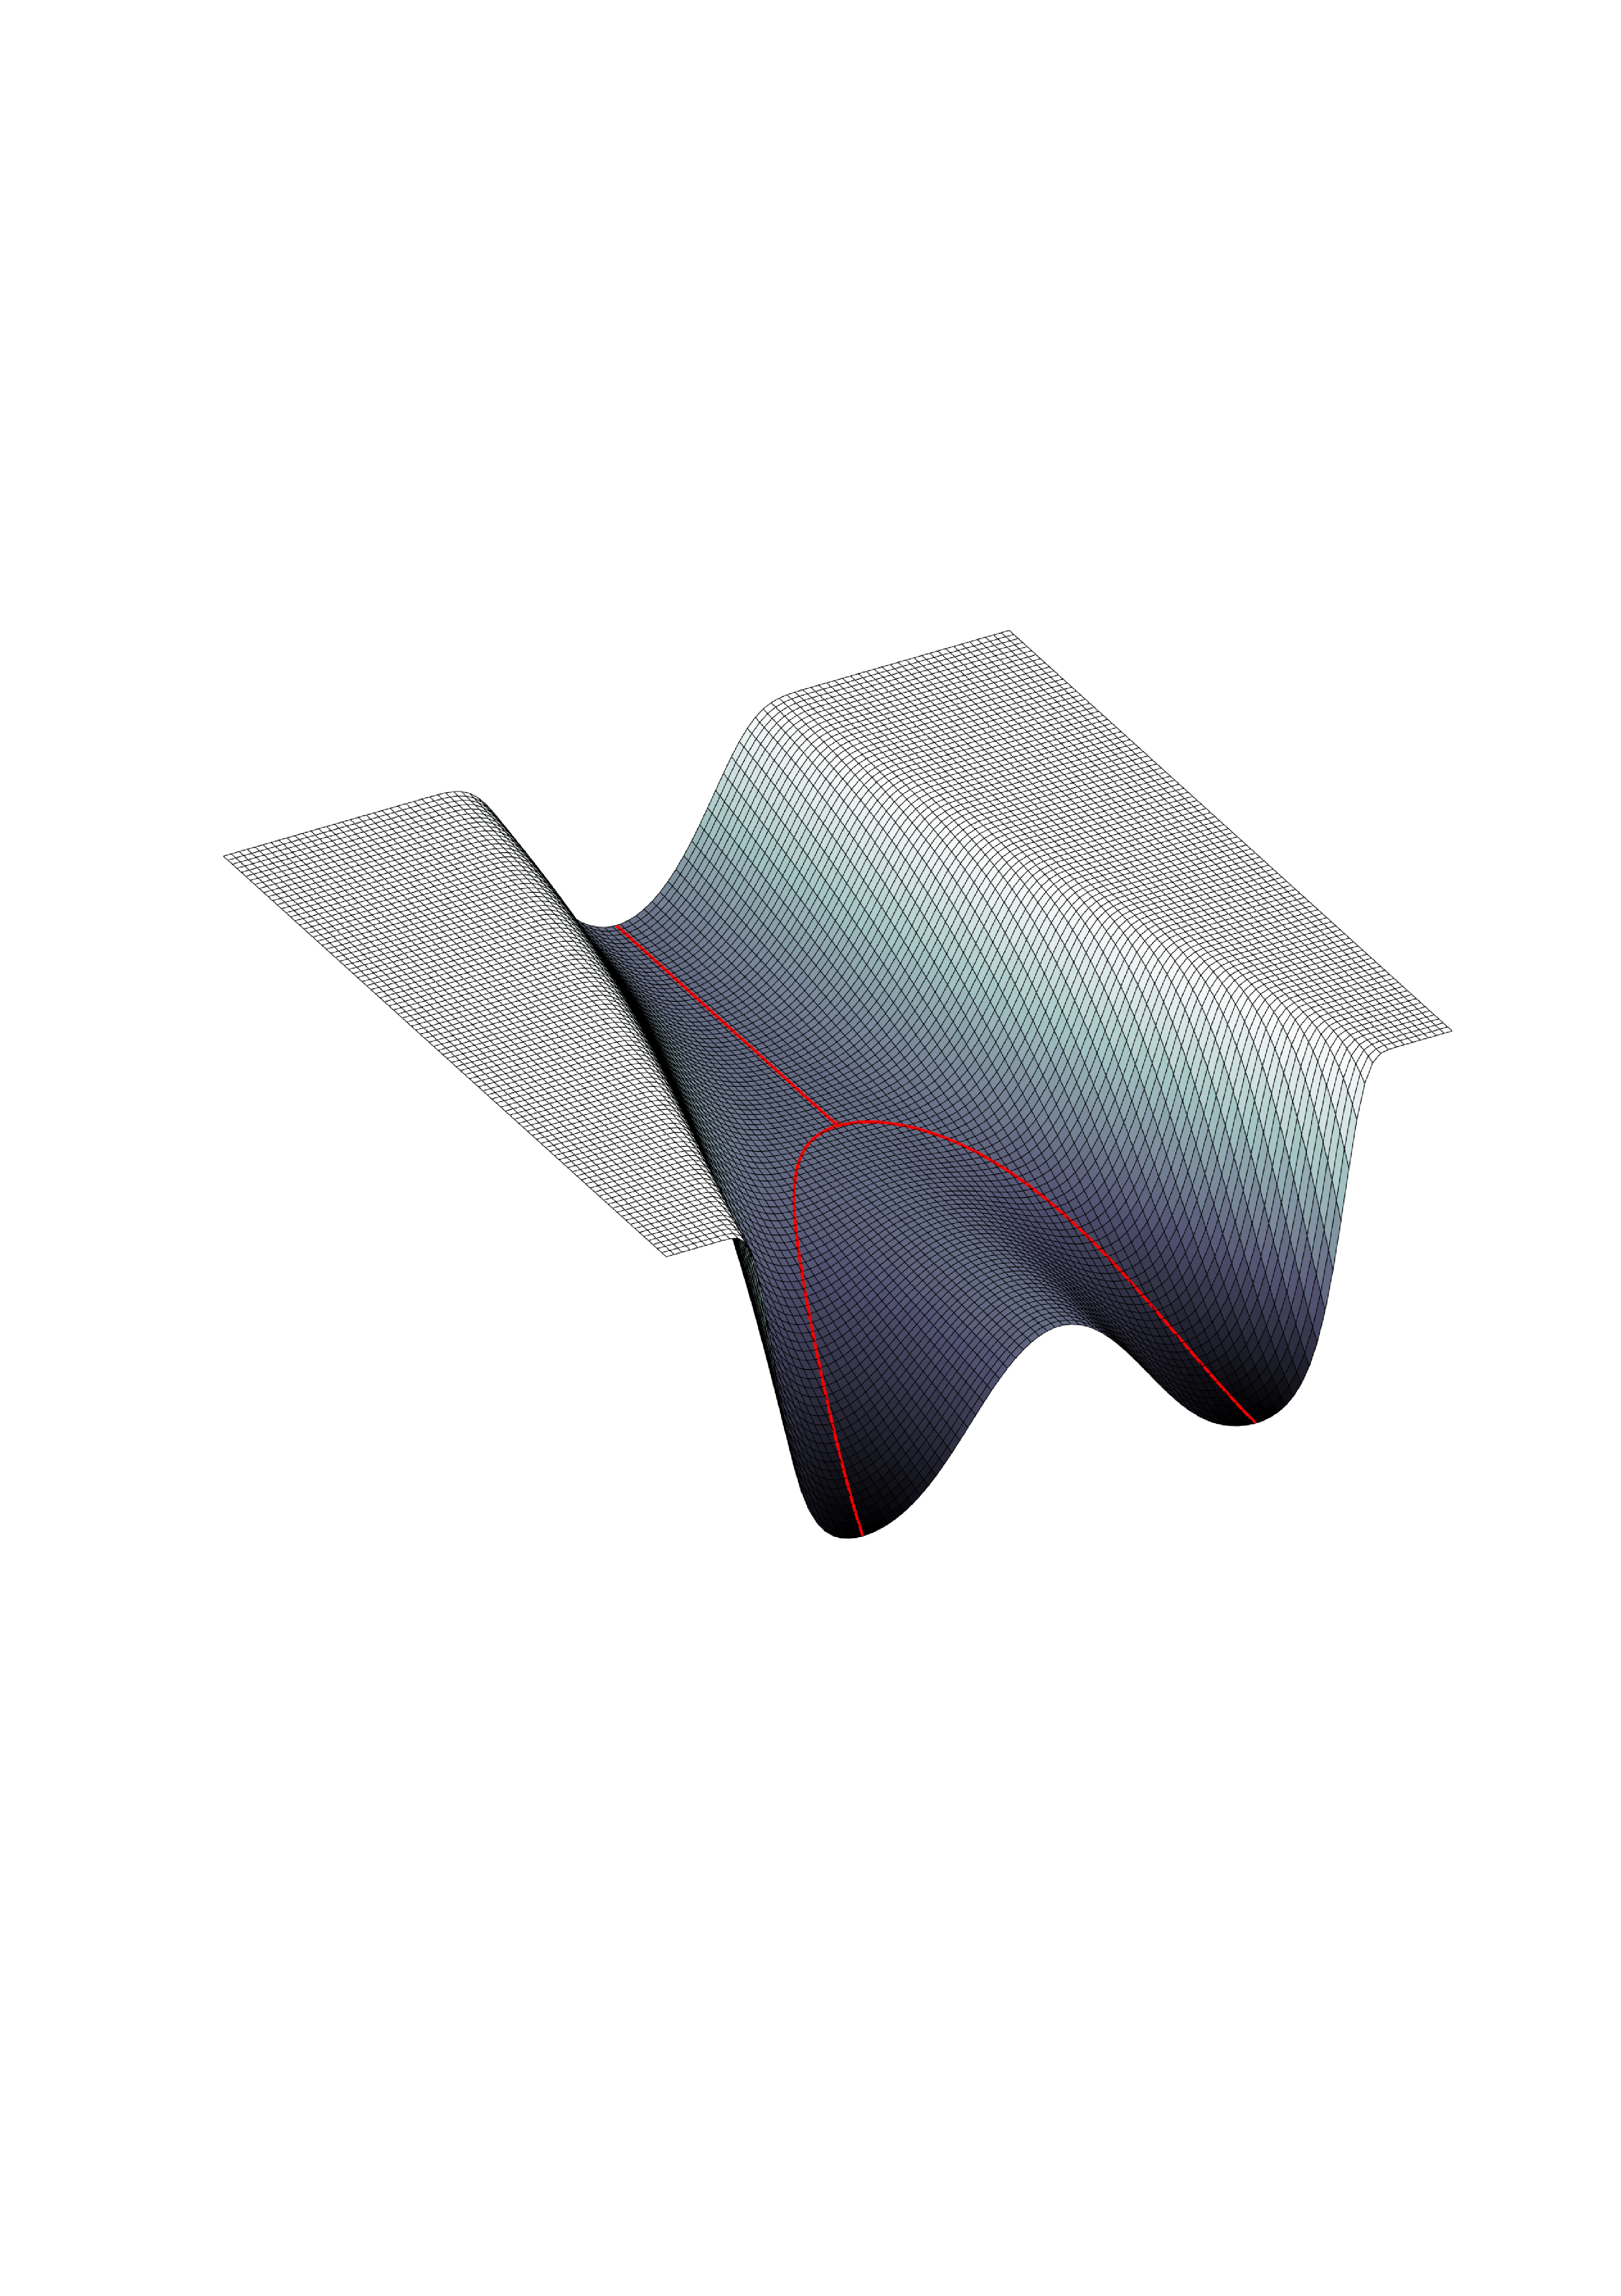
\includegraphics[width=\linewidth,trim={8cm 27cm 6cm 23cm},clip]{./surface2.pdf}
\end{column}

\begin{column}{0.5\columnwidth}
\begin{itemize}
\item Waddington describes cell specialisation like marbles rolling down a valley
\item When the valley splits, two cell fates emerge
\item This is a nice example of a bifurcation!
\end{itemize}
\end{column}
\end{columns}
\end{frame}

\begin{frame}[label={sec:org32b3f5a}]{Biological bifurcations}
\begin{columns}
\begin{column}{0.5\columnwidth}
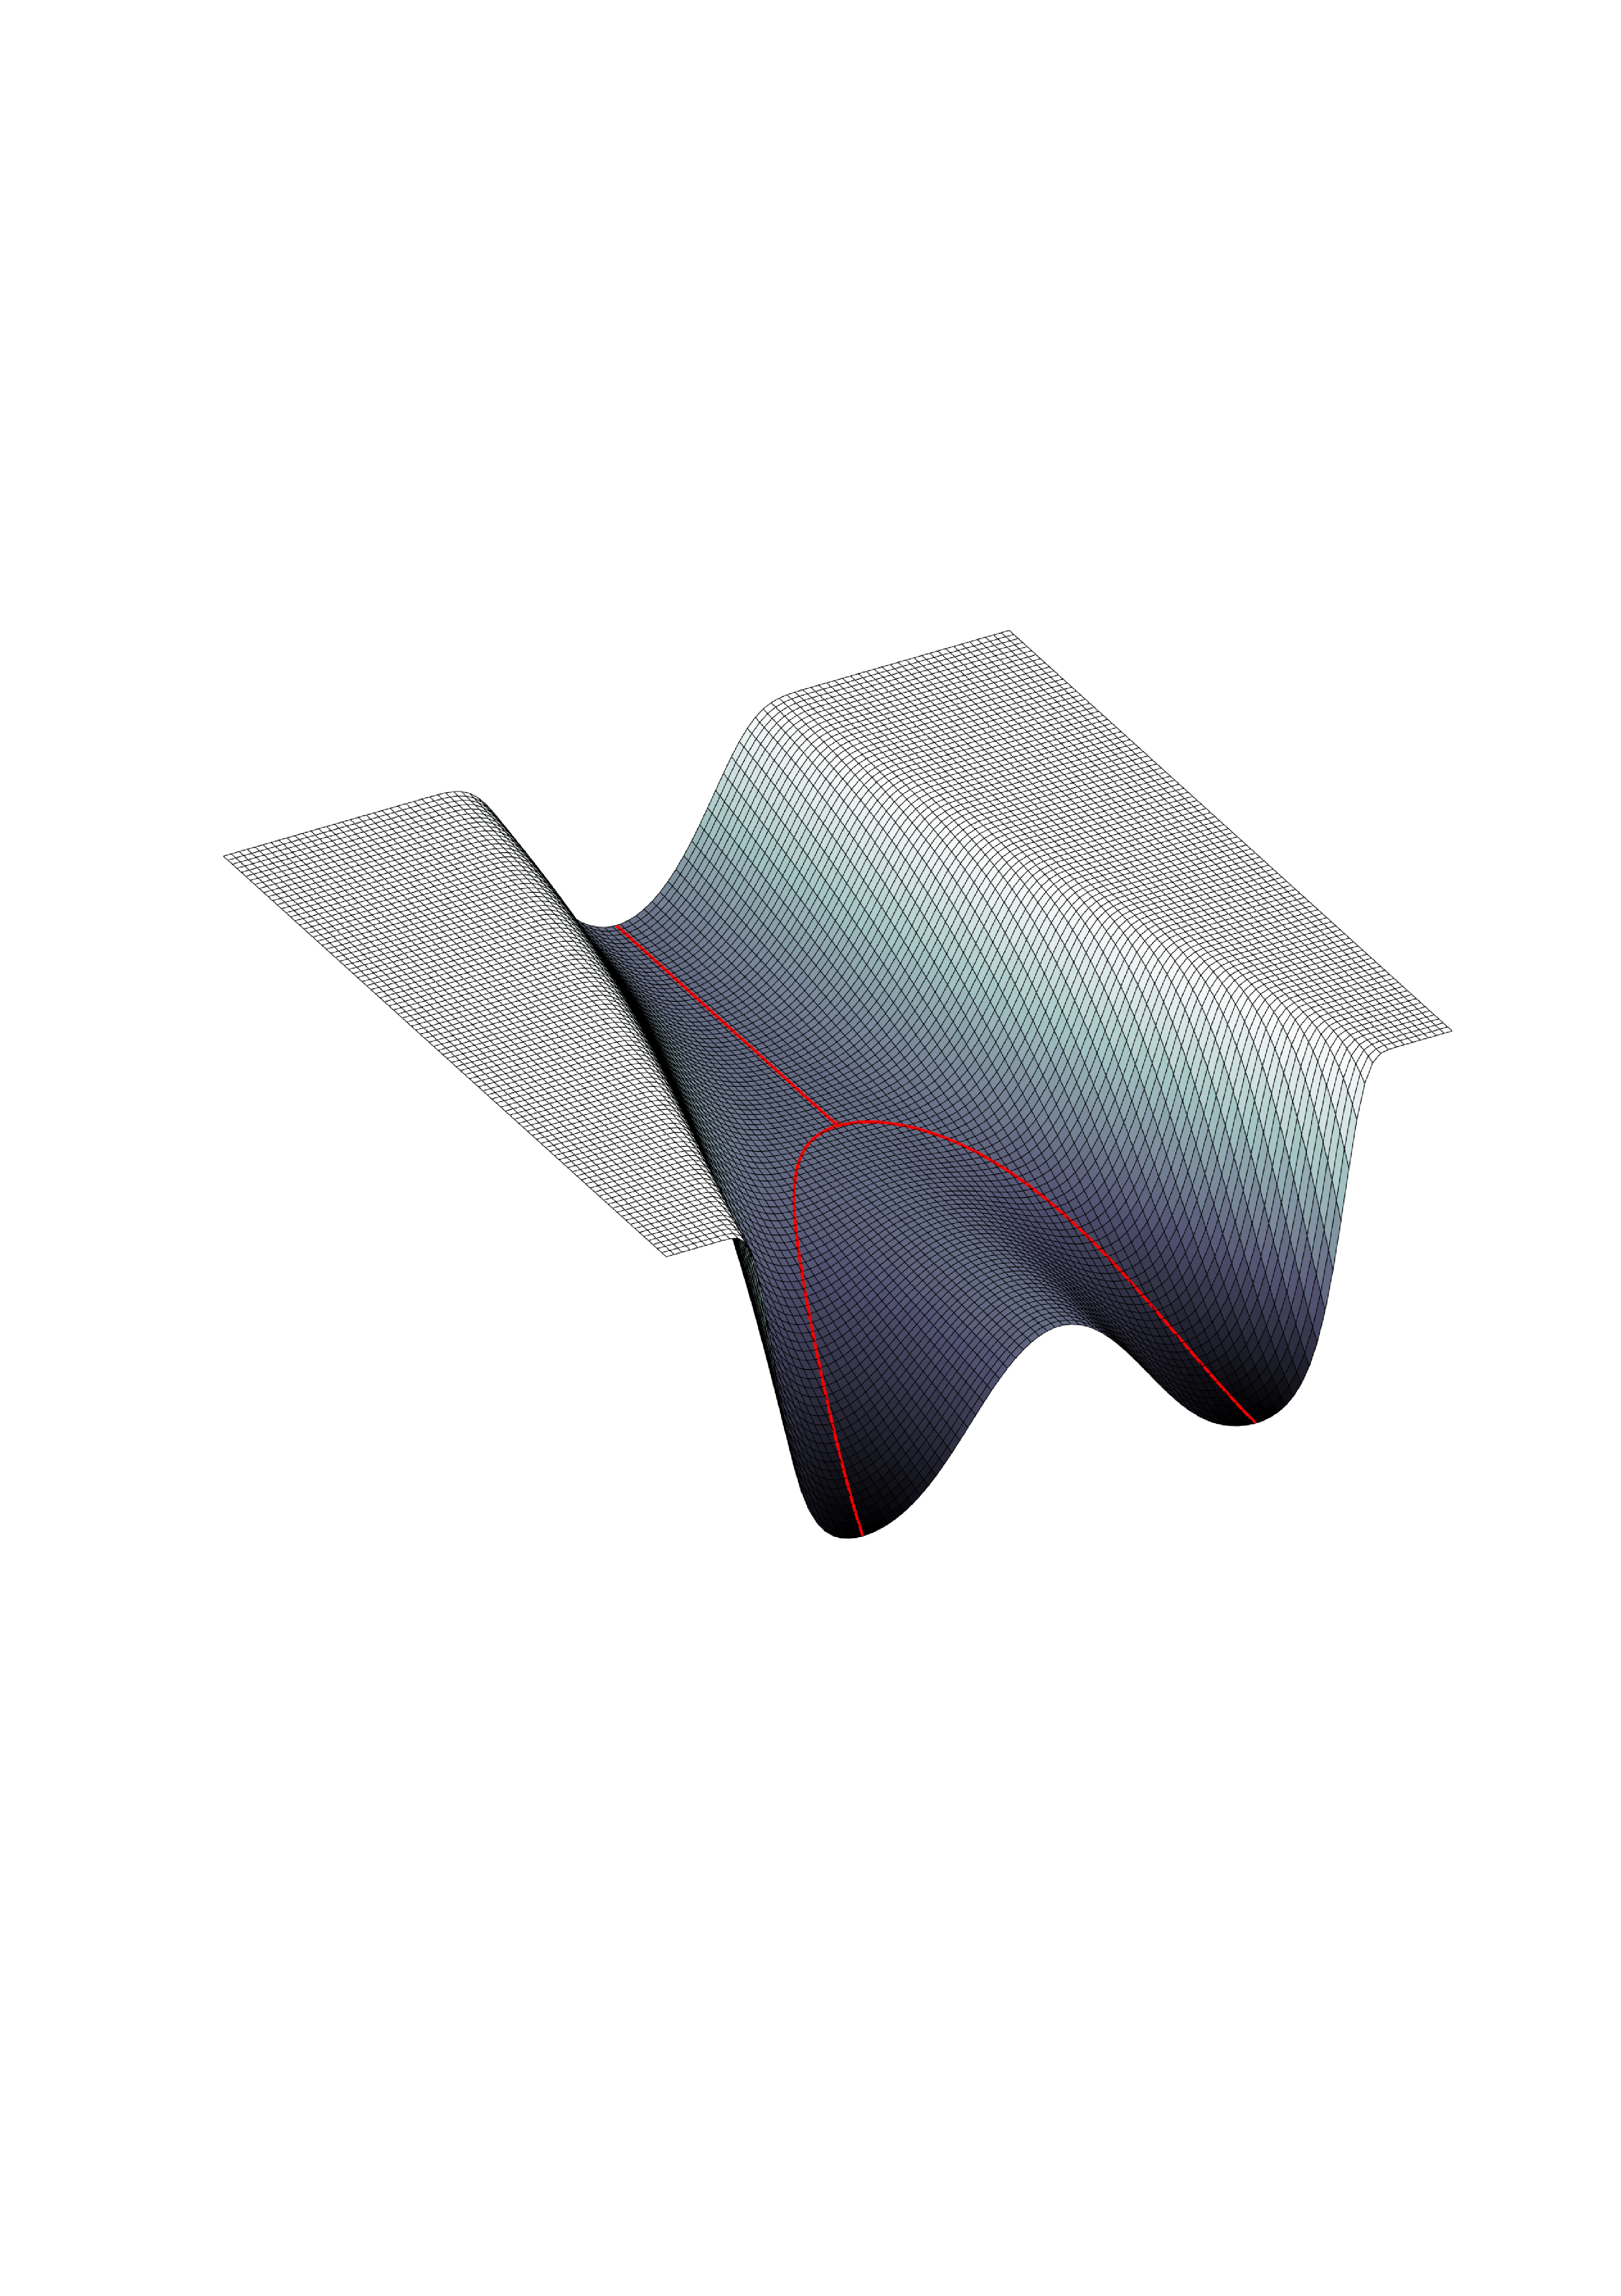
\includegraphics[width=\linewidth,trim={8cm 27cm 6cm 23cm},clip]{./surface2.pdf}
\end{column}

\begin{column}{0.5\columnwidth}
\begin{center}
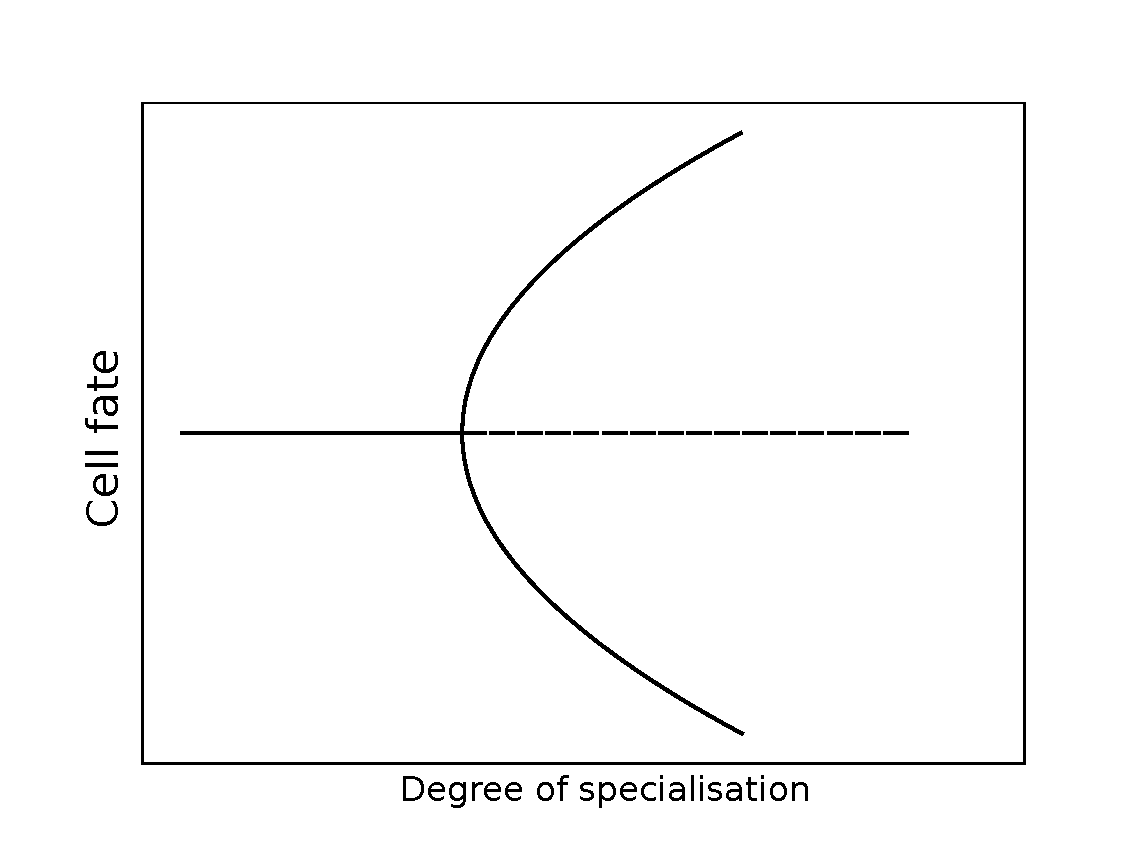
\includegraphics[width=.9\linewidth]{./pitchfork.pdf}
\end{center}
\end{column}
\end{columns}
\end{frame}

\begin{frame}[label={sec:orgfa560e9}]{The role of bifurcation analysis in biology}
\begin{itemize}
\item Bifurcations can explain seisures, heart attacks, Parkinson's, and many other diseases
\item Bifurcations can be used to explain the functionality of biological systems
\item Bifurcations can be used to design biological systems
\end{itemize}
\end{frame}

\begin{frame}[label={sec:org4a9ea15}]{Methods for bifurcation analysis}
\begin{itemize}
\item Analytical calculations
\item Brute force computation
\item Numerical continuation
\end{itemize}
\end{frame}

\begin{frame}[label={sec:org8bb8765}]{Numerical continuation}
\begin{itemize}
\item We use numerical continuation to track `interesting' points
\begin{itemize}
\item We vary a parameter
\item Continuation tells us how the point changes
\end{itemize}
\item Test functions indentify bifurcations
\end{itemize}
\end{frame}

\section{Chapter 2}
\label{sec:org084ec99}
\begin{frame}[label={sec:org476dbea}]{Bifurcation analysis of a bursting neuron}
\begin{center}
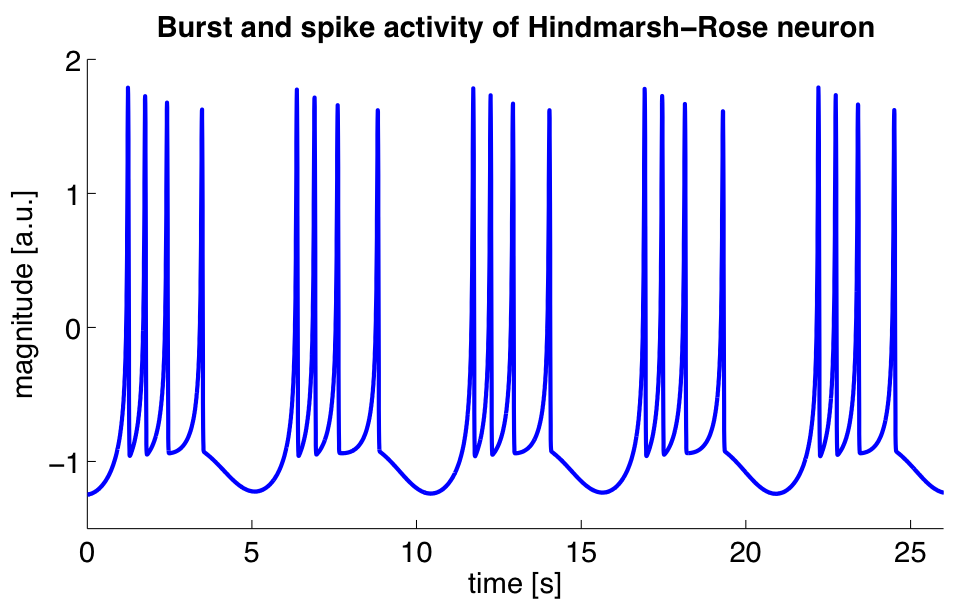
\includegraphics[height=.85\textheight]{./wikipedia_HR.png}
\end{center}
\end{frame}
\begin{frame}[label={sec:org02f14f4}]{The Hindmarsh Rose model}
\begin{align}
\frac{\mathrm{d} x}{\mathrm{d} t} &= y - ax^3 +bx^2 -z + I~,\\ \nonumber
\frac{\mathrm{d} y}{\mathrm{d} t} &= c- dx^2 -y~,\\ 
\frac{\mathrm{d} z}{\mathrm{d} t} &= r\left[s(x-x_R)-z\right]~.\nonumber
\end{align}

\vfill

\begin{center}
\(|r| \ll 1\)
\end{center}
\end{frame}
\begin{frame}[label={sec:orgd8703ec}]{Exploratory step}
\begin{center}
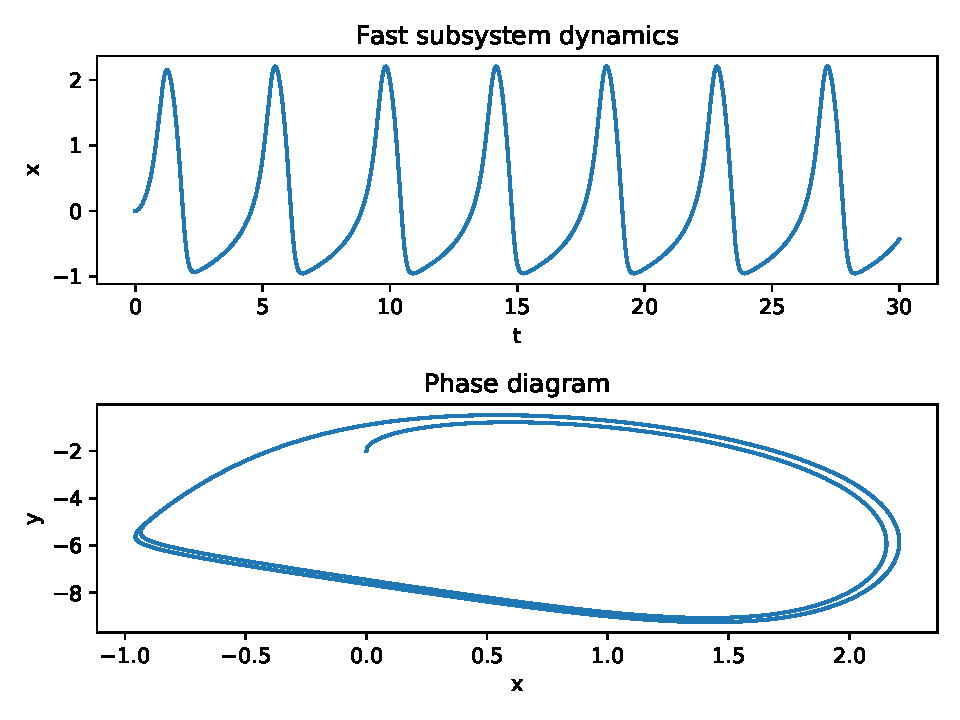
\includegraphics[height=.85\textheight]{./trajectory.pdf}
\end{center}
\end{frame}

\begin{frame}[label={sec:orgcd2ab6c}]{Initialisation step}
\begin{center}
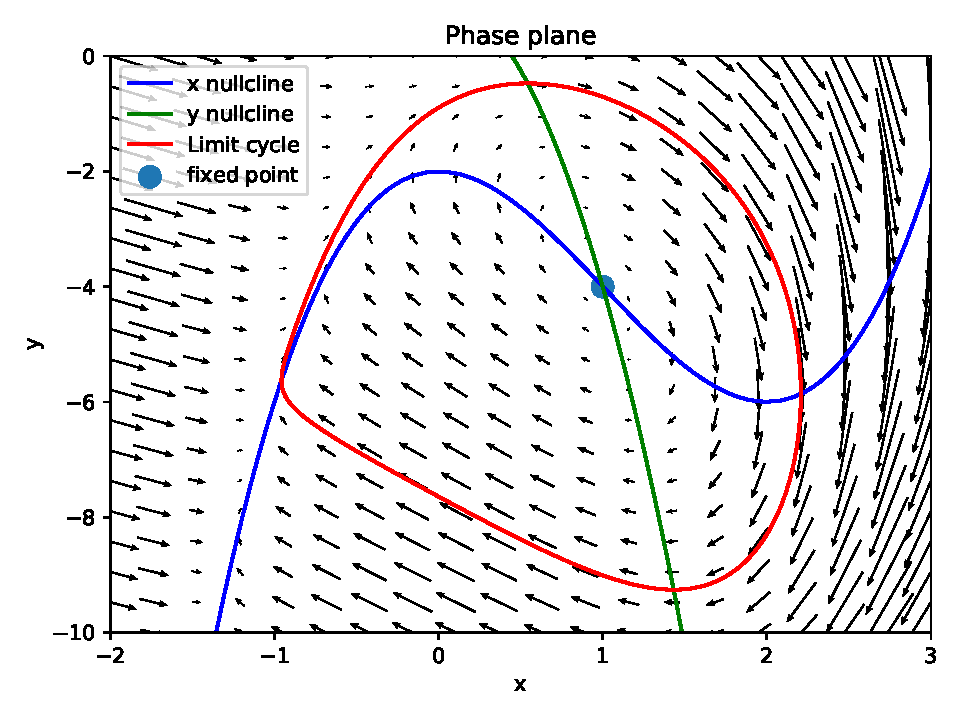
\includegraphics[height=.9\textheight]{./phaseplane.pdf}
\end{center}
\end{frame}
\begin{frame}[label={sec:orge46931d}]{Equilibrium point curve}
\begin{center}
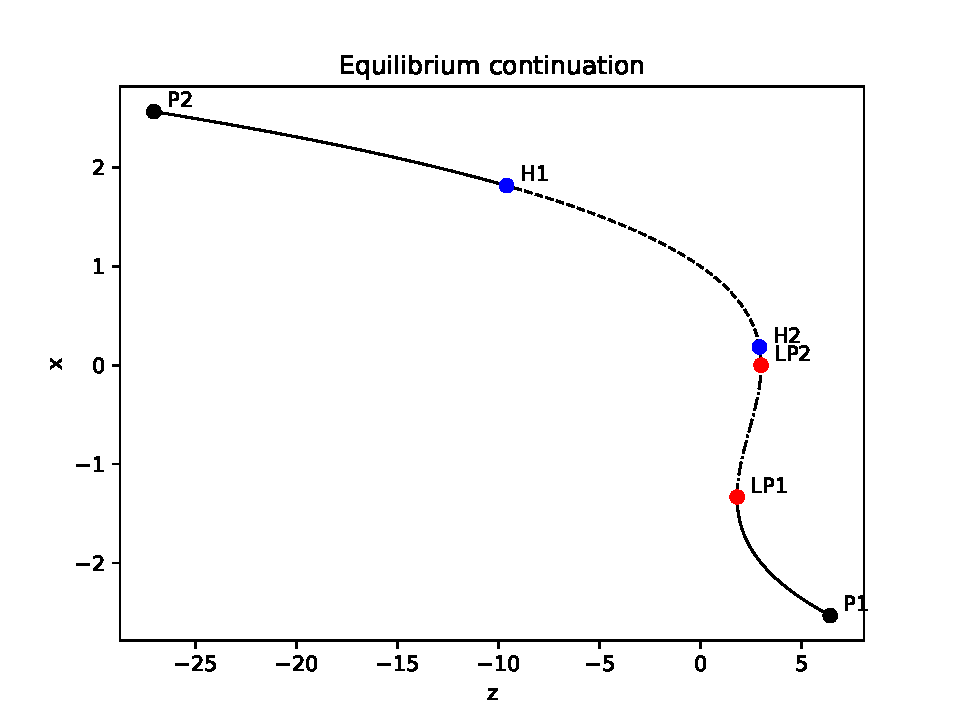
\includegraphics[height=.9\textheight]{./epc-1.pdf}
\end{center}
\end{frame}
\begin{frame}[label={sec:org805587b}]{Periodic orbit continuation}
\begin{center}
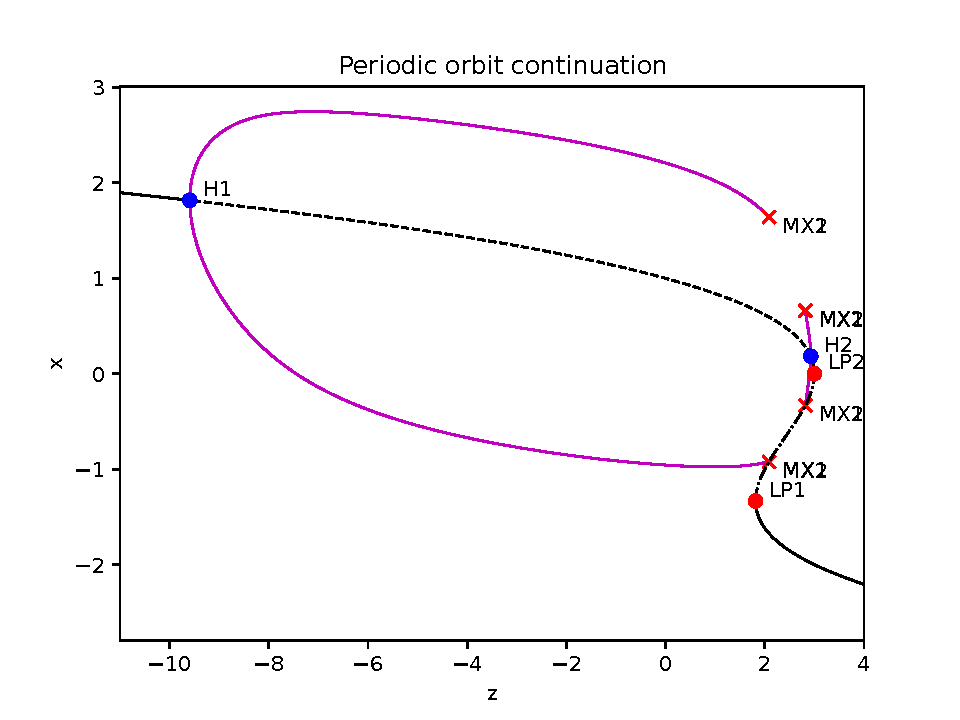
\includegraphics[height=.9\textheight]{./epc-2.pdf}
\end{center}
\end{frame}

\begin{frame}[label={sec:org5d9dbd5}]{Full system dynamics}
\begin{center}
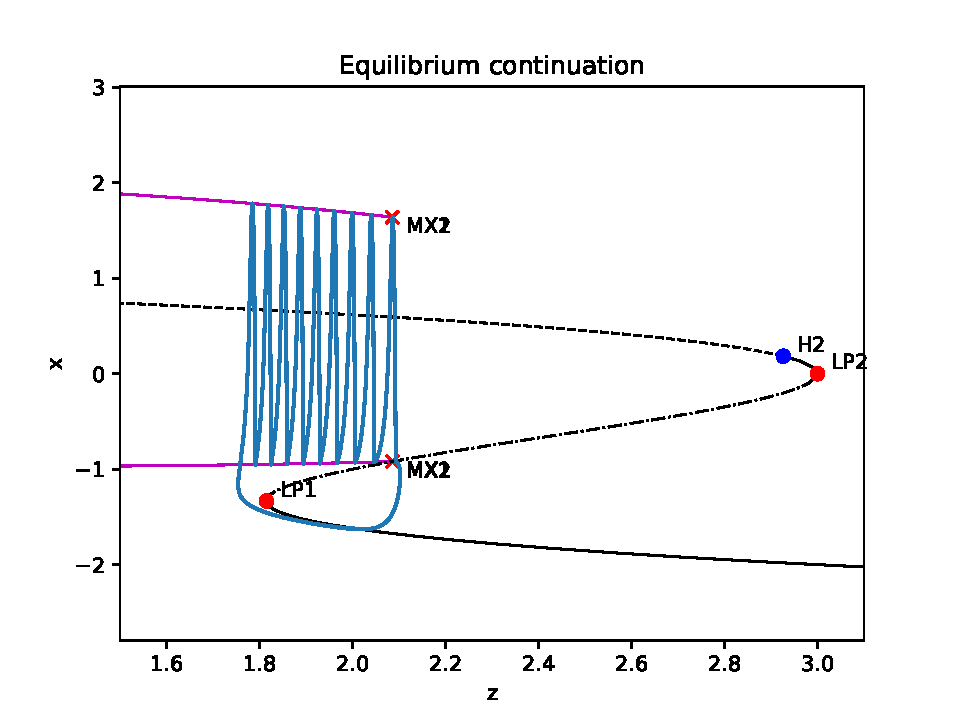
\includegraphics[height=.9\textheight]{./burster_diagram.pdf}
\end{center}
\end{frame}

\section{Chapter 3}
\label{sec:orgece099e}
\begin{frame}[label={sec:org54c31b8}]{Software tools}
There's lots of software to do these sorts of calculations!
\end{frame}

\section{End}
\label{sec:org03291ff}
\begin{frame}[label={sec:orgf568cca}]{}
\begin{center}
Questions? Feedback?
\end{center}
\end{frame}
\end{document}
